\everymath{\displaystyle}
\documentclass{beamer}
% \documentclass[handout]{beamer}

%\usepackage[pdftex]{color,graphicx}
\usepackage{amsmath,amssymb,amsfonts}

\mode<presentation>
{
  % \usetheme{Darmstadt}
  % \usetheme[hideothersubsections]{Hannover}
  % \usetheme[hideothersubsections]{Goettingen}
  \usetheme[hideothersubsections, right]{Berkeley}

  \usecolortheme{seahorse}
  % \usecolortheme{dolphin}
  \usecolortheme{rose}
  % \usecolortheme{orchid}

  \useinnertheme[shadow]{rounded}

  \setbeamercovered{transparent}
  % or whatever (possibly just delete it)
}

\mode<handout>{
  \setbeamercolor{background canvas}{bg=black!5}
  \usepackage{pgfpages}
  \pgfpagesuselayout{4 on 1}[a4paper,border shrink=5mm, landscape]
}

\usepackage[brazilian]{babel}
% or whatever

% \usepackage[latin1]{inputenc}
\usepackage[utf8]{inputenc}
% or whatever

\usepackage{times}
%\usepackage[T1]{fontenc}
% Or whatever. Note that the encoding and the font should match. If T1
% does not look nice, try deleting the line with the fontenc.


\title%[] % (optional, use only with long paper titles)
{Tópicos de busca bibliográfica}

\subtitle
{Google-fu et al} % (optional)

\author%[] % (optional, use only with lots of authors)
{Felipe Figueiredo}% \and S.~Another\inst{2}}
% - Use the \inst{?} command only if the authors have different
%   affiliation.

\institute[INTO] % (optional, but mostly needed)
{Instituto Nacional de Traumatologia e Ortopedia
}
  % \inst{1}%
  % Department of Computer Science\\
  % University of Somewhere
  % \and
  % \inst{2}%
  % Department of Theoretical Philosophy\\
  % University of Elsewhere}
% - Use the \inst command only if there are several affiliations.
% - Keep it simple, no one is interested in your street address.

\date%[] % (optional)
{}

% \subject{Talks}
% This is only inserted into the PDF information catalog. Can be left
% out. 



% If you have a file called "university-logo-filename.xxx", where xxx
% is a graphic format that can be processed by latex or pdflatex,
% resp., then you can add a logo as follows:

\pgfdeclareimage[height=1.6cm]{university-logo}{../logo}
\logo{\pgfuseimage{university-logo}}



% Delete this, if you do not want the table of contents to pop up at
% the beginning of each subsection:
\AtBeginSubsection[]
%\AtBeginSection[]
{
  \begin{frame}<beamer>{Sumário}
    \tableofcontents[currentsection,currentsubsection]
  \end{frame}
}


% If you wish to uncover everything in a step-wise fashion, uncomment
% the following command: 

\beamerdefaultoverlayspecification{<+->}


\begin{document}

\begin{frame}
  \titlepage
\end{frame}

\begin{frame}{Sumário}
  \tableofcontents
  % You might wish to add the option [pausesections]
\end{frame}


%% Template
% \section{}

% \subsection{}

% \begin{frame}{}
%   \begin{itemize}
%   \item 
%   \end{itemize}
% \end{frame}

% \begin{frame}
%   \begin{columns}
%     \begin{column}{5cm}
%     \end{column}
%     \begin{column}{5cm}
%     \end{column}
%   \end{columns}
% \end{frame}

% \begin{frame}{}
%   \includegraphics[height=0.4\textheight]{file1}
%   \includegraphics[height=0.4\textheight]{file2}
%   \includegraphics[height=0.4\textheight]{file3}
%   \begin{figure}
%     \caption{}
%   \end{figure}
% \end{frame}

% \begin{frame}{}
%   \begin{definition}
%   \end{definition}
%   \begin{example}
%   \end{example}
%   \begin{block}{Exercício}
%   \end{block}
% \end{frame}

\section{Bases bibliográficas}

\subsection{Google Scholar}

\subsection{PUBMED}

\subsection{Web of Science}

\section{Google-fu}

\subsection{Google Books}

\begin{frame}{Google Books}
  \begin{itemize}
  \item Plataforma \alert{Google
      Books}\footnote{\url{https://books.google.com/}} (antes: Google
    Book Search e Google Print)
  \item Iniciado em 2004, digitalizou milhões de livros + OCR para
    extrair a íntegra do texto
  \item Tem 4 níveis de acesso para o acervo:
    \begin{enumerate}
    \item Full view (domínio público)
    \item Preview (\% disponível, escolha da editora)
    \item Snippet view (2--3 linhas em torno da chave de busca)
    \item No preview
    \end{enumerate}
  \end{itemize}
\end{frame}

\begin{frame}{Buscando livros no Google Books}
  Pode-se \ldots
  \begin{itemize}
  \item localizar livros buscando por:
    \begin{itemize}
    \item Metadados (autor(es) e/ou título)
    \item Trechos ou frases
    \end{itemize}
  \item consultar preview ou a íntegra (se disponível em domínio
    público)
  \item \alert{exportar} informações bibliográficas\footnote{arquivo
      .RIS} para \alert{importação} no Mendeley (\ldots, Endnote,
    etc.)
  \end{itemize}
\end{frame}

\begin{frame}{Busca por metadados}
  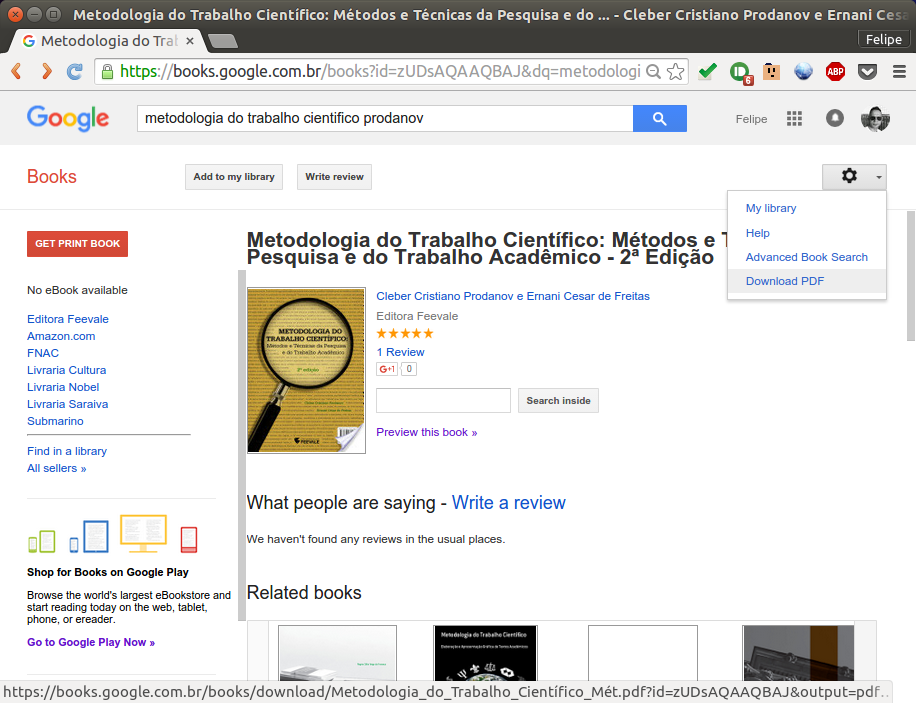
\includegraphics[height=.85\textheight]{Busca/gbooks-livro}

\end{frame}

\begin{frame}{Preview}
  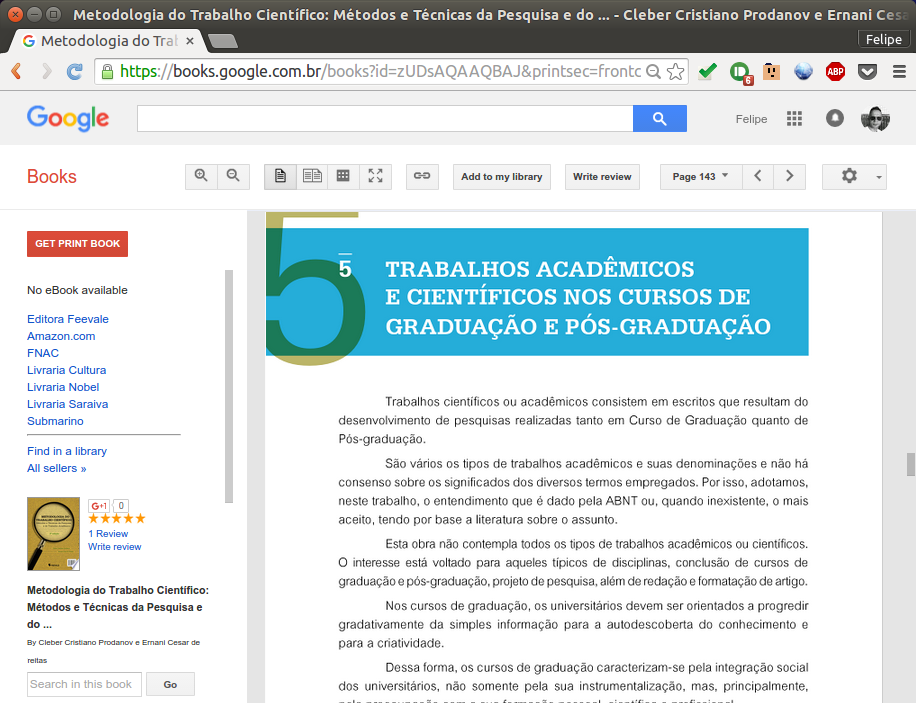
\includegraphics[height=.85\textheight]{Busca/gbooks-preview}
\end{frame}

\begin{frame}{Domínio Público}
  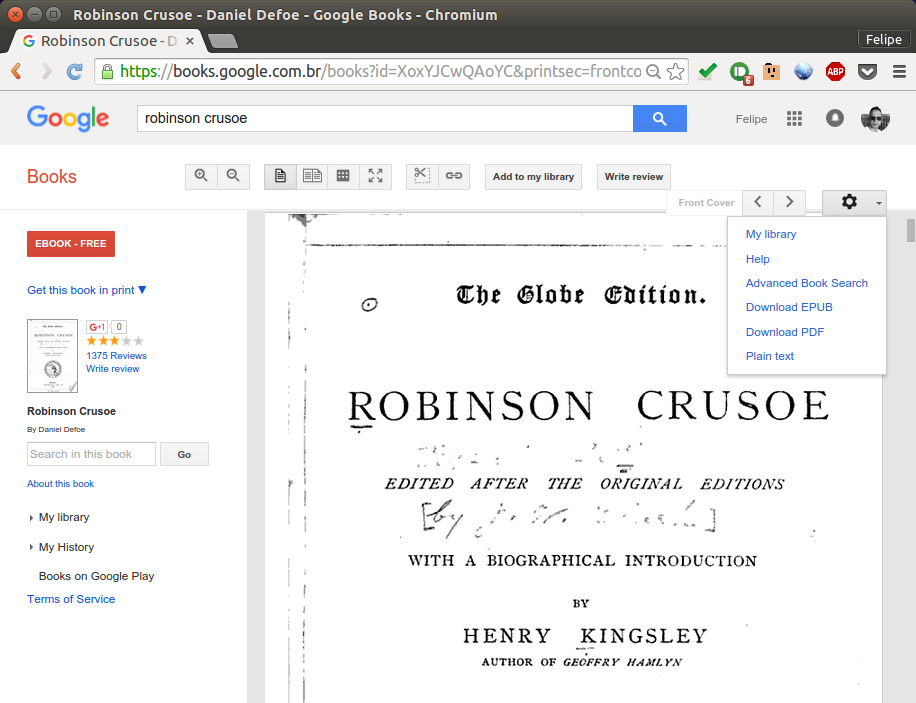
\includegraphics[height=.85\textheight]{Busca/gbooks-publicdomain}
\end{frame}

\begin{frame}{Livros acadêmicos}
  \begin{itemize}
  \item Estamos interessados em livros acadêmicos/científicos
  \item Ao fazer, e.g., uma citação direta, podemos usar o Google
    Books para:
    \begin{itemize}
    \item localizar o livro
    \item importar a referência para nosso gerenciador de refs
    \end{itemize}
  \end{itemize}
  \begin{example}[Buscando a frase\ldots]
    ``Life depends on the ability of cells to store, retrieve, and
    translate the genetic instructions required to make and maintain a
    living organism.''
  \end{example}
\end{frame}

\begin{frame}{Busca por conteúdo}
  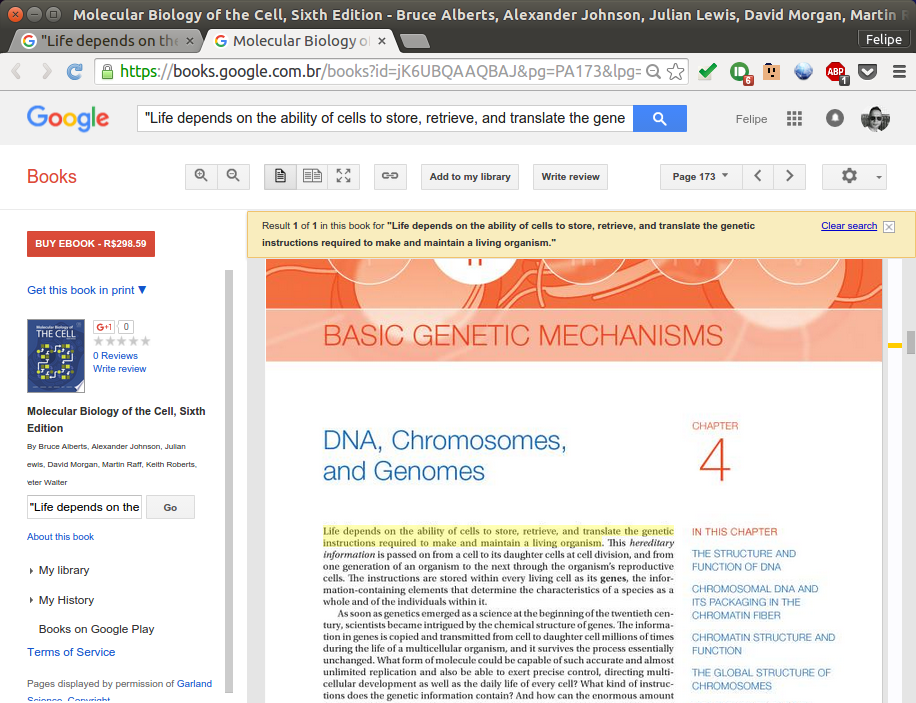
\includegraphics[height=.85\textheight]{Busca/gbooks-busca-conteudo}
\end{frame}

\begin{frame}{Importando a referência}
  \begin{itemize}
  \item Seção ``Sobre este Livro'' ({\em About this book} na coluna
    esquerda do slide anterior)
  \item Ao pé da página, temos todas as informações bibliográficas, e
    opções para baixar como arquivo
  \item A opção do arquivo .RIS (RefMan) pode ser importada pelo
    Mendeley
  \end{itemize}
\end{frame}

\begin{frame}{Sobre este livro}
  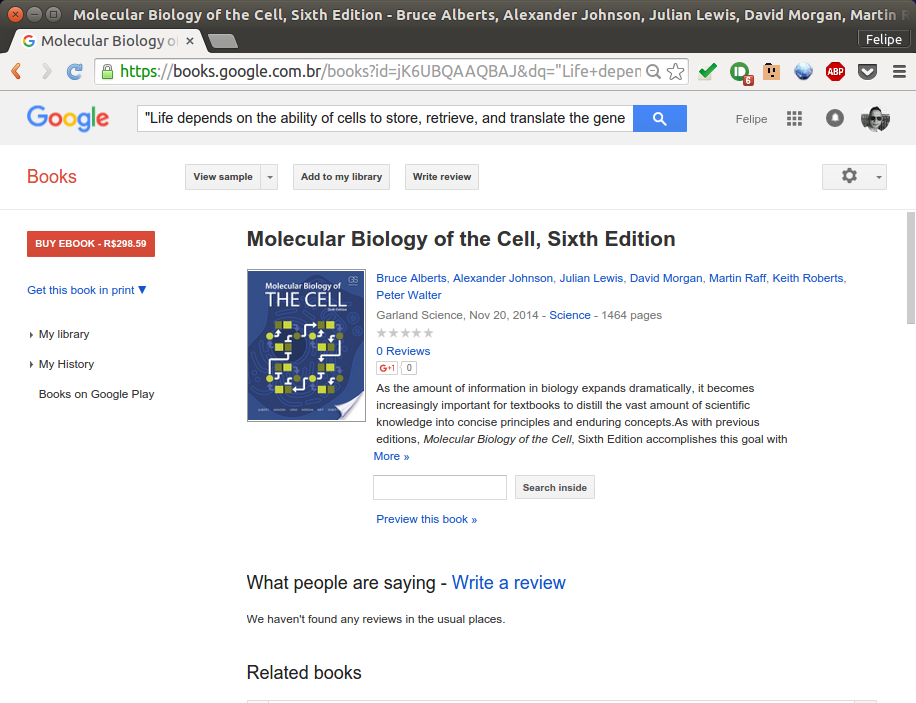
\includegraphics[height=.85\textheight]{Busca/gbooks-about1}
\end{frame}

\begin{frame}{Exportar arquivo RIS (RefMan)}
  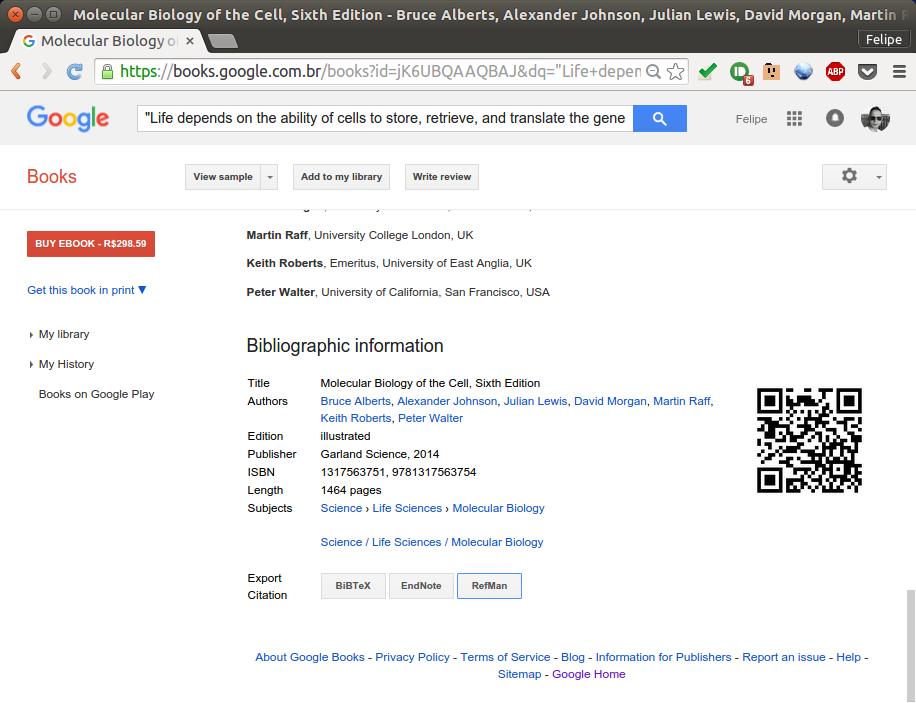
\includegraphics[height=.85\textheight]{Busca/gbooks-about2}
\end{frame}

\section{Deep Web}

\subsection{Papers}

\subsection{Livros}

\end{document}
